\subsection{Saving the Measurement Results Automatically}

When you have a time series sequence and you want to measure multiple signals with 
multiple parameters in each frame, measurement results in each frame needs to be somehow saved. 
Here, we learn how to export measurement results in your hard disk automatically using macro. 

Open the sample image \ilcom{Nucseq001.tif}. Cell nucleus shows that they divide and 
increase their number over time. We want to count the number of nucleus in each frame to know 
the dynamics of increase. 
At the same time, we may also want to see changes in the signal intensity and shape. 
For this measurement Particle Analysis function works best. Do the following:

\begin{enumerate}
\small{
\item \ijmenu{[Image -> Adjust -> Threshold]}. 
Threshold the image and check the threshold lower and upper value that segments the nucleus optimally. 
\item Set the measurement parameters. \ijmenu{[Analysis -> set measurements\ldots]}
\begin{enumerate}
\item Check Area, Mean intensity, centroid, Circularity and Slice number. 
\item Check "limit to threshold"
\item Digits after decimal point: 2
\end{enumerate}
\item \ijmenu{[Analyze -> Analyze Particles\ldots]}
\begin{enumerate}
\item Size: 10 - Infinity
\item Circularity = 0.5 - 1.0
\item Show: Outline
\item Check Display Results
\item Check Exclude on Edges
\item Check Clear Results
\end{enumerate}
\item Then click "OK". 
}
\end{enumerate}
After these steps, you will find outline image showing detected cells and a result table. 

%double figure
\begin{figure}[htbp]
 \centering
 \subfloat[]{\label{fig:thresholdCells}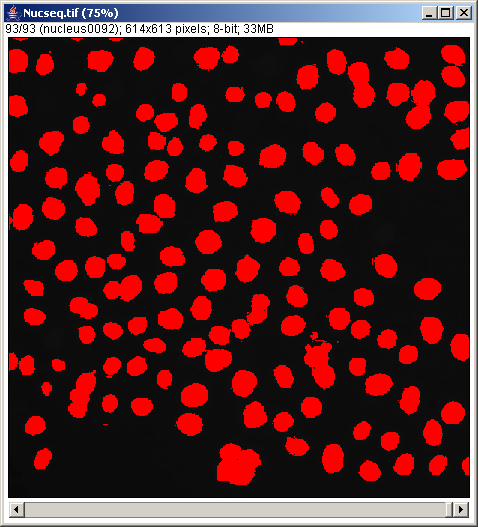
\includegraphics[height = 60mm]{fig/fig2511a_CellsThreshold.png}}
 \subfloat[]{\label{fig:ParticleAnalysisDialog}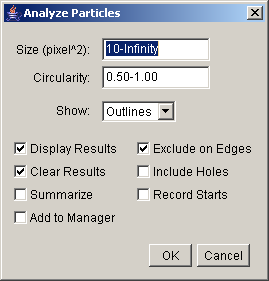
\includegraphics[height = 60mm]{fig/fig2511b_AnalyzeParticleDialog.png}}
 \caption{ (a) Thresholded cell image and (b) Particle Analysis parameter input dialog.}
 \label{fig:ParticleAnalysis}
\end{figure}

%double figure
\begin{figure}[htbp]
 \centering
 \subfloat[]{\label{fig:OutlinedCells}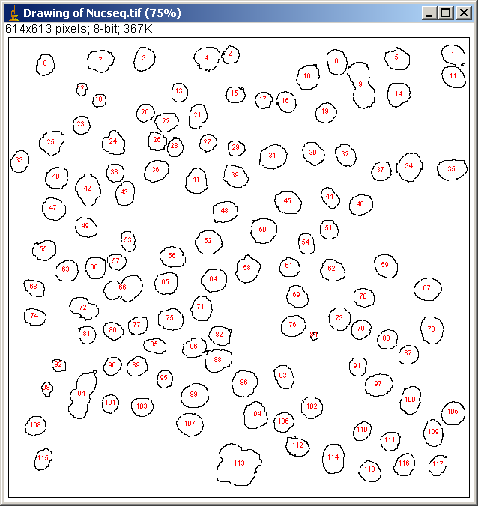
\includegraphics[height = 50mm]{fig/fig2511c_CellOutlines.png}}
 \subfloat[]{\label{fig:ParticleAnalysisResults}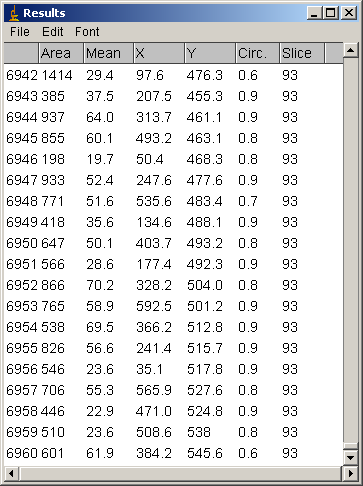
\includegraphics[height = 50mm]{fig/fig2511d_ParticleAnalysisResults.png}}
 \caption{ After particle analysis is done, (a) outlined cell image and (b) results table listing measurement results.}
 \label{fig:ParticleAnalysisResults}
\end{figure}

Using macro recorder, its easy to write a macro set as following. 

\lstinputlisting[morekeywords={*, }]{code/code21.ijm}

Two macros and a global variable consists this macro set. 
Global variable is a string variable that stores the path to the location where file will be saved. 
(note: path is differently written in MacOS. It uses slash instead of back-slash). 
The first macro \ilcom{Set Directory to save Results} is for setting the path to the folder 
(or directory) where the file will be saved. 
We use a macro function \ilcom{getDirectory(title)} to get user choice of a destination folder. 

\begin{indentCom}
\textbf{getDirectory(title)}\\
Returns the path to a specified directory. If title is "startup", returns the path to the directory 
that ImageJ was launched from (usually the ImageJ directory). If it is "plugins" or 
"macros", returns the path to the plugins or macros folder. If it is "image", 
returns the path to the directory that the active image was loaded from. 
If it is "home", returns the path to users home directory. 
If it is "temp", returns the path to the /tmp directory. 
Otherwise, displays a dialog (with title as the title), 
and returns the path to the directory selected by the user. 
Note that the path returned by getDirectory() ends with a file separator, 
either "\" (Windows) or "/". Returns an empty string if the specified directory is not found or 
aborts the macro if the user cancels the dialog box.
\end{indentCom}

When you run this first macro, global string variable \ilcom{G\_Ddir} 
will be set to a folder where user will select, and line 6 prints out the path to 
a folder (or directory). It might be convenient for you to change the default directory path 
in the code above (line 2), by copying the results in the log window and pasting it in the macro. 

The measurement macro starts from the Line 9. 
\begin{itemize}
\item Line 10 to 13: Checks if the image is thresholded. 
\item Line 14: Sets the threshold level. 
\item Line 15: Gets the title of the image window for later use. We use this for 
generating name of the results file.
\item Line 16: to 17: Sets the measurement parameter and does the actual 
particle analysis. Macro functions are direct copies from the recorder. 
\end{itemize}
After the analysis, we want to save the results. 
\begin{itemize}
\item Line 18: Generates the file name using the image file name stored in the line 15 by concatenating concatenate image title with \ilcom{\_measure.xls}. 
\item Line 19: The full path file name is constructed by adding the result filename generated in line 18 with path stored in the global variable. 
\item Line 20: Saving the result table as an excel-readable file uses a new macro function \ilcom{saveAs}:
\begin{indentCom}
\textbf{saveAs(format, path)}
Saves the active image, lookup table, selection, measurement results, selection XY coordinates or text window to the specified file path. The format argument must be "tiff", "jpeg", "gif", "zip", "raw", "avi", "bmp", "fits", "png", "pgm", "text image", "lut", "selection", "measurements", "xy Coordinates" or "text". Use saveAs(format) to have a "Save As" dialog displayed.
\end{indentCom}
Path in line 20 is a full path constructed in the previous line 19.
\end{itemize}

\begin{indentexercise}{1}
Create a new macro file and write the code 21. If it works, save the macro as "macro\_fileIO.ijm". We use it in the next section (.ijm is the extension for imageJ macro). 
Then modify the code so that user can change the size-range for the particle analysis. Save the file separately.   
\end{indentexercise}
